% PLAM-2026 theme on a white canvas: light colours, vector Percona Live logo,
% white arrow interior. \input after \usetheme{plam-2026}.

% light variant: white canvas, dark text (plam-2026 is dark by default, and
% \usecolortheme{percona-2026} is a no-op here since the theme already loaded it)
\setbeamercolor*{normal text}{fg=percona-2026black,bg=white}
\setbeamercolor*{background canvas}{bg=white}
\setbeamercolor*{frametitle}{fg=percona-2026black}
\setbeamercolor*{itemize item}{fg=percona-2026black}
\setbeamercolor*{itemize subitem}{fg=percona-2026black}
\setbeamercolor*{itemize subsubitem}{fg=percona-2026black}
\setbeamercolor*{itemize/enumerate body}{fg=percona-2026black}
\setbeamercolor*{itemize/enumerate subbody}{fg=percona-2026black}
\setbeamercolor*{itemize/enumerate subsubbody}{fg=percona-2026black}
\setbeamercolor*{enumerate item}{fg=percona-2026black}
\setbeamercolor*{enumerate subitem}{fg=percona-2026black}

% theme loads moreverb but never uses it, drop its listing envs so minted can define its own
\makeatletter
\expandafter\let\csname listing\endcsname\@undefined
\expandafter\let\csname endlisting\endcsname\@undefined
\expandafter\let\csname listing*\endcsname\@undefined
\expandafter\let\csname endlisting*\endcsname\@undefined
\makeatother
\usepackage{minted}
\usetikzlibrary{calc}

\graphicspath{{./theme/images/}}

\pgfplotsset{compat=1.18}

\setminted{fontsize=\footnotesize,style=default}

% same as the plam-2026 frametitle template, but title box ends before the
% triangle decoration (0.85\paperwidth) so long titles wrap instead of overflowing,
% and the arrow's inner triangle is white to match the canvas
\setbeamertemplate{frametitle}{
  \begin{textblock*}{\paperwidth}(0pt,0pt)
    \tikz[remember picture,overlay] {%
      \draw[fill=percona-2026blue,percona-2026blue] (0\paperwidth,-0.76\paperheight) -- (0.07\paperwidth,-1\paperheight) -- (0\paperwidth,-1\paperheight) -- cycle;
    }
  \end{textblock*}

  \begin{textblock*}{\paperwidth}(0.85\paperwidth,0\paperheight)
    {
\includegraphics[width=0.18\paperwidth,keepaspectratio]{plam2026_slide.png}}
  \end{textblock*}

  \begin{tikzpicture}[overlay, remember picture]
    \begin{scope}[shift={(current page.north west)}]
      \draw[fill=percona-2026blue,percona-2026blue] (0.021\paperwidth,-0.128\paperheight) -- (0.054\paperwidth,-0.160\paperheight) -- (0.021\paperwidth,-0.191\paperheight) -- cycle;
      \draw[fill=white,white] (0.025\paperwidth,-0.137\paperheight) -- (0.048\paperwidth,-0.160\paperheight) -- (0.025\paperwidth,-0.182\paperheight) -- cycle;
    \end{scope}
  \end{tikzpicture}

  \begin{textblock*}{0.78\paperwidth}(0.06\paperwidth,0.12\paperheight)
    \begin{beamercolorbox}[left, wd=0.78\paperwidth]{frametitle}
      \usebeamerfont{title in head/foot}\insertframetitle
    \end{beamercolorbox}%
  \end{textblock*}
}

% same as the percona-2026 title page template, but with the vector logo
% instead of the low-res png
\setbeamertemplate{title page}{
  \begin{textblock*}{\paperwidth}(0\paperwidth,0\paperheight)
    {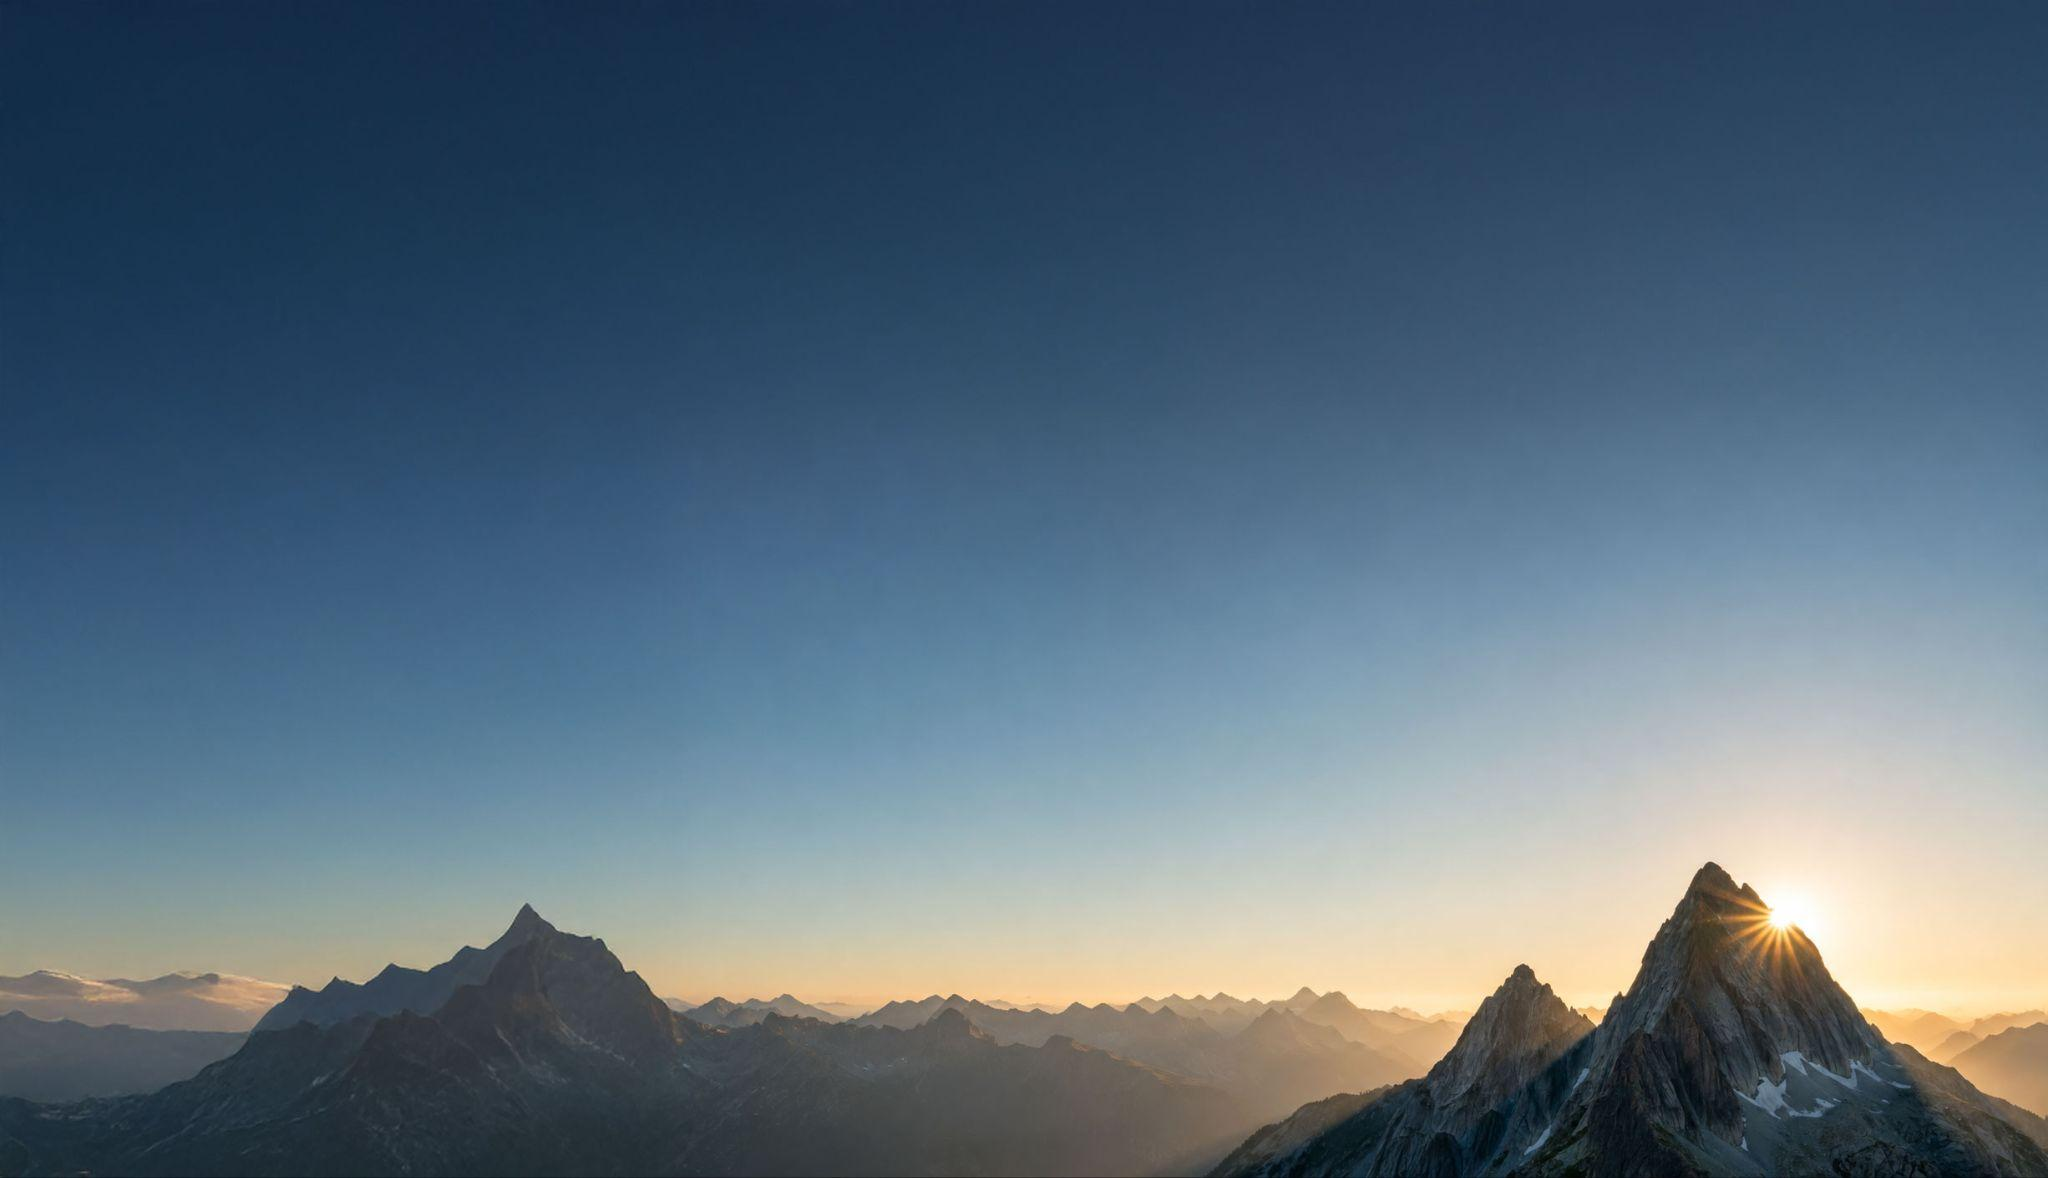
\includegraphics[width=\paperwidth,keepaspectratio]{plam2026_title.jpg}}
  \end{textblock*}

  \begin{textblock*}{\paperwidth}(0\paperwidth,0\paperheight)
  \begin{tikzpicture}[overlay, remember picture]
    \begin{scope}[shift={(current page.north west)}]
      \draw[fill=percona-2026black,percona-2026black] (0.078\paperwidth,0\paperheight) -- (\paperwidth,0\paperheight) -- (0.675\paperwidth,-1\paperheight) -- (0\paperwidth,-1\paperheight) -- (0\paperwidth,-0.245\paperheight) -- cycle;
      \draw[fill=percona-2026yellow,percona-2026yellow] (0\paperwidth,0\paperheight) -- (0.078\paperwidth,0\paperheight) -- (0\paperwidth,-0.245\paperheight) -- cycle;

      \draw[fill=percona-2026blue,percona-2026blue] (0.341\paperwidth,-0.666\paperheight) -- (0.374\paperwidth,-0.698\paperheight) -- (0.341\paperwidth,-0.729\paperheight) -- cycle;
      \draw[fill=percona-2026black,percona-2026black] (0.345\paperwidth,-0.675\paperheight) -- (0.368\paperwidth,-0.698\paperheight) -- (0.345\paperwidth,-0.720\paperheight) -- cycle;
    \end{scope}
  \end{tikzpicture}
  \end{textblock*}

  \begin{textblock*}{0.48\paperwidth}(0.32\paperwidth,0.125\paperheight)
    \begin{beamercolorbox}{title page header}
      \usebeamerfont{title}\inserttitle\hfill%
    \end{beamercolorbox}%
  \end{textblock*}

  \begin{textblock*}{0.353\paperwidth}(0.38\paperwidth,0.64\paperheight)
    \begin{beamercolorbox}{author}
      {\usebeamerfont{author}\insertauthor}\hfill\par\usebeamerfont{institute}\insertinstitute\hfill\par\usebeamerfont{date}\insertdate\hfill%
    \end{beamercolorbox}%
  \end{textblock*}

  \begin{textblock*}{\paperwidth}(0.06\paperwidth,0.222\paperheight)
    {\includegraphics[width=0.222\paperwidth,keepaspectratio]{perconalive_light.pdf}}
  \end{textblock*}
}

% theme footline logo is white text, invisible on white canvas: use the dark variant instead
\setbeamertemplate{footline}{
  \ifnum \insertpagenumber=1
  \else
    \begin{textblock*}{\paperwidth}(0.85\paperwidth,0.7\paperheight)
      {\includegraphics[width=0.1\paperwidth,keepaspectratio]{perconalive.pdf}}
    \end{textblock*}

    \begin{textblock*}{\paperwidth}(0.025\paperwidth,0.95\paperheight)
      \begin{beamercolorbox}{framenumber}
        \usebeamerfont{framenumber}\insertpagenumber%
      \end{beamercolorbox}%
    \end{textblock*}

    \begin{textblock*}{\paperwidth}(0.85\paperwidth,0.95\paperheight)
      \begin{beamercolorbox}{copyright}
        \usebeamerfont{copyright}\textcopyright~\the\year~Percona
      \end{beamercolorbox}%
    \end{textblock*}

    \vskip0.3in%
  \fi
}

% Template \tyslide needs social icon images missing from the repo, so build the slide by hand
\newcommand{\thankyouslide}{
{
\usebackgroundtemplate{
\includegraphics[width=\paperwidth,keepaspectratio]{ty_bg.jpg}}
\setbeamertemplate{footline}{}
\begin{frame}[plain]
  \begin{textblock*}{\paperwidth}(0pt,0pt)
    \tikz[remember picture,overlay] {%
      \draw[fill=percona-2026blue,percona-2026blue] (0.922\paperwidth,0\paperheight) -- (1\paperwidth,0\paperheight) -- (\paperwidth,-0.245\paperheight) -- cycle;
    }
  \end{textblock*}

  \begin{textblock*}{\paperwidth}(0pt,0.38\paperheight)
    \centering
    {\usebeamerfont{title}\color{percona-2026white}Thank you!}
  \end{textblock*}

  \begin{textblock*}{\paperwidth}(0.790\paperwidth,0.87\paperheight)
    {
\includegraphics[width=0.18\paperwidth,keepaspectratio]{percona_one_color_light.png}}
  \end{textblock*}
\end{frame}
}
}
